\begin{frame}{Grafos Outerplanares}
    \begin{minipage}{\linewidth}
        \centering
        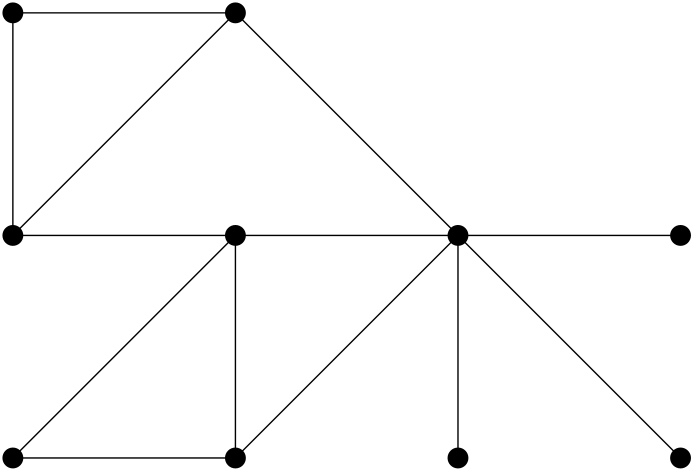
\includegraphics[height=5cm]{images/outerplanar.png}
    \end{minipage}
\end{frame}

\begin{frame}{Grafos $k$-outerplanares}
    \centering
    \Large Exemplo para $k=3$:
    \bigbreak
    \begin{minipage}{\linewidth}
        \centering
        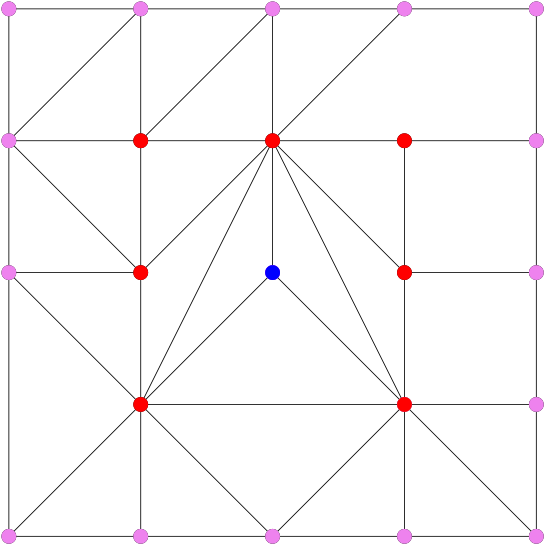
\includegraphics[height=6cm]{images/k-outer.png}
    \end{minipage}
\end{frame}

\begin{frame}{CI em Grafos $k$-outerplanares}
    \begin{lema}[1] \label{lema1}
        Existe um algoritmo por PD que resolve CI em grafos $k$-outerplanares em tempo $2^{O(k)} \cdot n$.
    \end{lema}
\end{frame}

\begin{frame}{Esboço da Prova}
    \begin{proof}
        \begin{lema}[\cite{Bod98}]
            Grafos $k$-outerplanares têm largura arbórea no máximo $3k - 1$.
        \end{lema}
        \bigbreak
        \begin{lema}[\cite{Cygan15}]
            Seja $G$ um grafo com $n$ vértices e largura arbórea $\leq k$. Então, CI em $G$ pode ser resolvido em tempo $2^k \cdot k^{O(1)} \cdot n$.
        \end{lema}
        \alt<3>{\qedhere}{\phantom\qedhere}
    \end{proof}
\end{frame}
